

Abschließend fließen nun die einzelnen Komponenten, welche durch entsprechende SIBs repräsentiert werden, in das Prozessmodell ein. Die folgende Abbildung \ref{fig:jabcmodel} zeigt das fertige Projektergebnis, welches die in Kapitel \ref{aufgabe} beschriebene Aufgabenstellung erfüllt.\\

\begin{figure}[h!t]
\begin{center}
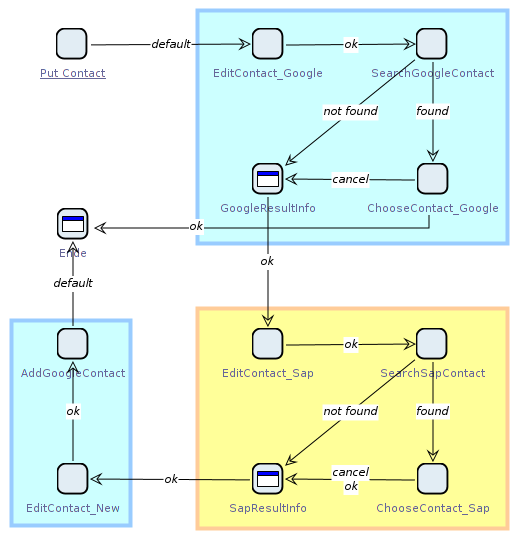
\includegraphics[width=0.5\textwidth]{Bilder/jabc_Model.png}
\end{center}
\caption{fertiges Prozessmodell im jABC}
\label{fig:jabcmodel} 
\end{figure} 

Zunächst lassen sich die farblich-gekennzeichneten Bereiche erkennen. Die blauen Bereiche enthalten die Kommunikation mit der Datenbank bei Google, während der gelbe Bereich die Kommunikation mit dem SAP-System repräsentiert. Die farbige Kennzeichnung dient auch der Tatsache, dass sich diese Bereiche in Untermodelle auslagern lassen, um diese z.B. in anderen Modellen wiederzuverwenden. Im Rahmen dieses Projektes wurde jedoch aus Gründen der Übersichtlichkeit darauf verzichtet. Ebenso verhält es sich mit den in Kapitel \ref{sibs_spez} beschriebenen \textit{error}-Branches. \\
Zudem ist die Wiederverwendung der SIBs erkennbar, welche für die Nutzereingabe verantwortlich sind und es fällt auf, dass die Struktur der Suchanfragen bei SAP und Google eine gemeinsame Struktur haben.


